\definecolor{BackendsColor}{RGB}{116,143,204}
\definecolor{AstColor}{RGB}{199,108,107}
\definecolor{ShapesColor}{RGB}{227,225,107}
\definecolor{UtilsColor}{RGB}{118,219,125}

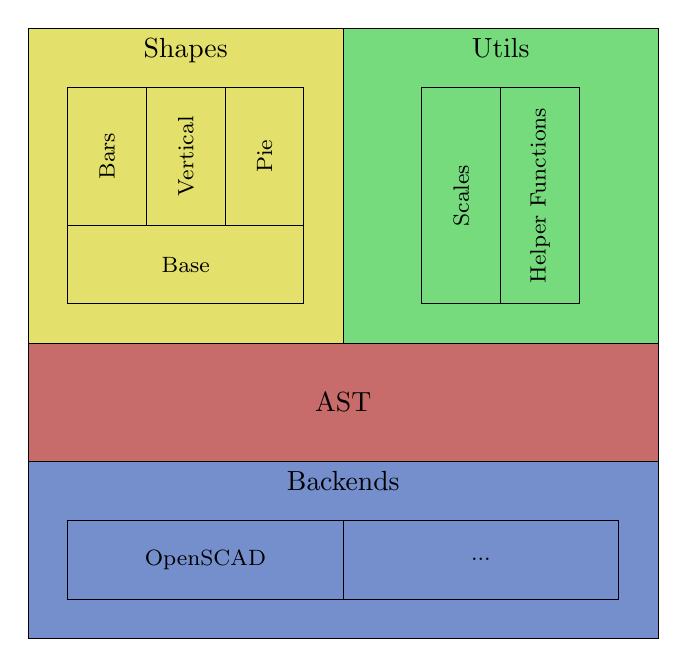
\begin{tikzpicture}

	% Main rectangles

	\filldraw [fill=BackendsColor] (0,-1.75) rectangle (8,0.5);
	\filldraw [fill=AstColor] (0,0.5) rectangle node [align=center] {AST} (8,2);
	\filldraw [fill=ShapesColor] (0,2) rectangle (4,6);
	\filldraw [fill=UtilsColor] (4,2) rectangle (8,6);

	% Inner rectangles

	\draw (0.5,2.5) rectangle node [font=\footnotesize] {Base} (3.5,3.5);
	\draw (0.5,3.5) rectangle node [rotate=90,font=\footnotesize] {Bars} (1.5,5.25);
	\draw (1.5,3.5) rectangle node [rotate=90,font=\footnotesize] {Vertical} (2.5,5.25);
	\draw (2.5,3.5) rectangle node [rotate=90,font=\footnotesize] {Pie} (3.5,5.25);

	\draw (5,2.5) rectangle node [rotate=90,font=\footnotesize] {Scales} (6,5.25);
	\draw (6,2.5) rectangle node [rotate=90,font=\footnotesize] {Helper Functions} (7,5.25);

	\draw (0.5, -1.25) rectangle node [font=\footnotesize] {OpenSCAD} (4, -0.25);
	\draw (4, -1.25) rectangle node [font=\footnotesize] {...} (7.5, -0.25);

	% Labels

	\node [below] at (2,6) {Shapes};
	\node [below] at (6,6) {Utils};
	\node [below] at (4,0.5) {Backends};

\end{tikzpicture}
